\section{Proposed Architecture}

\subsection{Overview}

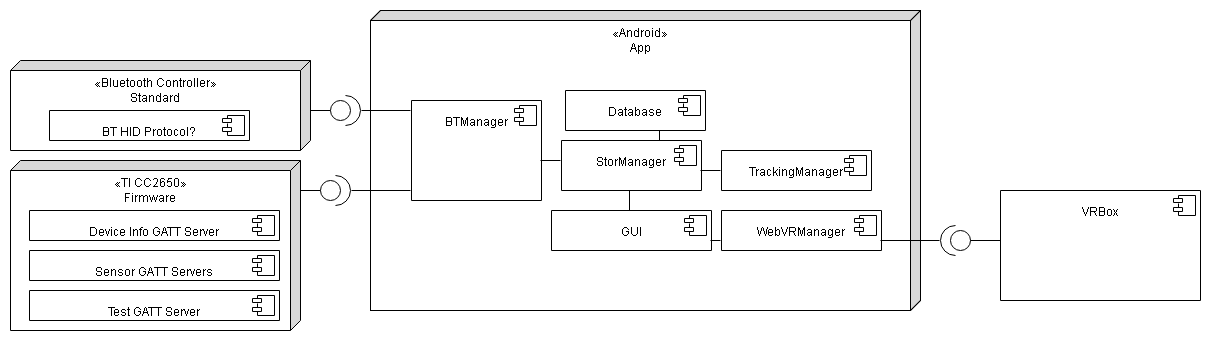
\includegraphics[scale=0.35]{pics/composite_app.png}

\subsection{Component Decomposition}

\subsubsection{Services}
From \href{https://developer.android.com/guide/components/services.html}{AndroidDoc}: \\
``A Service is an application component that can perform long-running operations in the background, and it does not provide a user interface''.
\begin{itemize}
  \item \textbf{BluetoothManager:} Uses the android.bluetooth and especially the android.bluetooth.le libraries to fetch the sensor data from the TI CC2650.
  \item \textbf{TrackingManager:} Handles the tracking of the cellphone and therefore of the TI SensorTag devices. the current position gets determined by GPS and enhanced by the cellphone sensor and wifi data.
  \begin{center}
  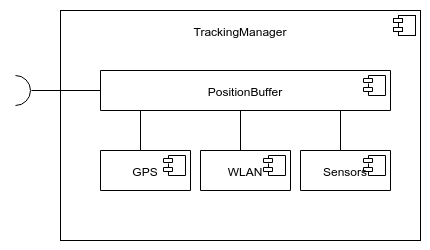
\includegraphics[scale=0.4]{pics/TrackingManager_Composition.png}
  \end{center}
  
  \item \textbf{WebVRManager:} Uses webview to display the WebVr-World and communicates with the WebVr-Site.
  \item \textbf{StorageManager:} Handles and processes the data provided by the TrackinManager and the BluetoothManager. Uses a DB to store processed Data.
  \begin{center}
  	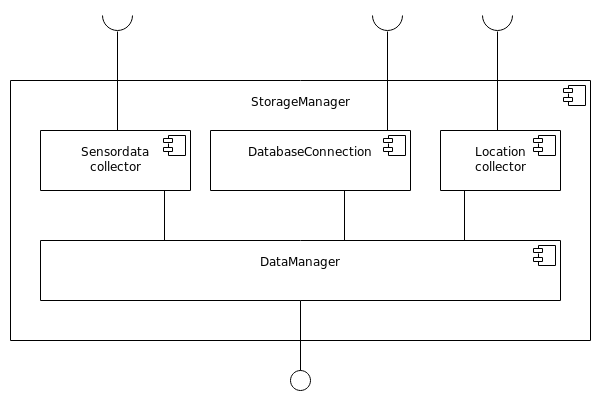
\includegraphics[scale=0.4]{pics/StorageMgr_Composition.png}
  \end{center}
  % (z.B. NeDB or internal stor or similar to safe parsed sensor input, location, settings,...)
  \item \textbf{VRBox:} Handles the display of the Vr-World and the given data from the sensor.
  \begin{center}
	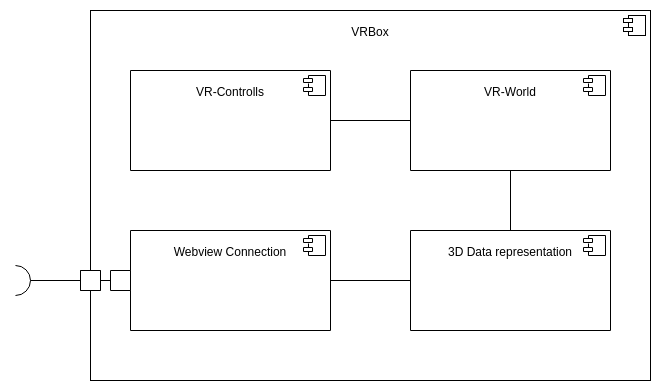
\includegraphics[scale=0.35]{pics/VRBox.png}
  \end{center}
\end{itemize}


\subsubsection{GUI}
From \href{https://developer.android.com/guide/components/services.html}{AndroidDoc}: \\
``They (Activities) serve as the entry point for a user's interaction with an app, and are also central to how a user navigates within an app (as with the Back button) or between apps (as with the Recents button)''. \newline
\begin{itemize}
  \item \textbf{MainActivity} Provides the main startup screen as the main entry point.
  \item \textbf{VRViewActivity} shall provide the WebVR view using the android.webkit library (especially .webview).
  \item \textbf{LiveDataActivity} shall provide a view of the sensor data in human readable form.
  \item \textbf{TISettingsActivity:} Settings screen containing scanning and connecting, connected devices and device settings fragments.
  \begin{itemize}
    \item \textbf{ScanningConnectingFragment} shall show the scanning results, delivered by the SensorTagBluetoothReceiverService and controll to which device to connect to or disconnect.
    \item \textbf{ConnectedDevicesFragment} shall show a list of all connected devices and a short info about the current setting and state of the TI SimpleLink SensorTag device.
    \item \textbf{ConnectedDevicesSettingsFragment} shall implement the configuration of the app features of the sensor.
  \end{itemize}
\end{itemize}

\subsubsection{Additional Classes}
\begin{itemize}
  \item \textbf{GATT Profiles} (for each sensor one)
  \item \textbf{GATT Sensor Service UUIDs}
  \item \textbf{Parser Functions} because the BLE protocol implemented in the TI CC2650 delivers raw sensor output
\end{itemize}
